\documentclass[conference]{IEEEtran}
\IEEEoverridecommandlockouts
\usepackage{cite}
\usepackage{amsmath,amssymb,amsfonts}
\usepackage{booktabs}
\usepackage{graphicx}
\usepackage{tikz}
\usepackage{pgfplots}
\pgfplotsset{compat=1.18}
\usetikzlibrary{arrows.meta,positioning,shapes.geometric,calc}
\usepackage{hyperref}

\def\BibTeX{{\rm B\kern-.05em{\sc i\kern-.025em b}\kern-.08em
    T\kern-.1667em\lower.7ex\hbox{E}\kern-.125emX}}

\begin{document}

\title{Speed and Torque Control of a Switched Reluctance Motor:
MATLAB/Simulink Implementation, Cubic TSF Ripple Minimisation,
and Independent Validation}

\author{%
\IEEEauthorblockN{Ahmed Mostafa}
\IEEEauthorblockA{\textit{Dept.\ of Mechatronics Engineering}\\
\textit{German University in Cairo}\\
Cairo, Egypt\\
Student ID: 55-1591}
\and
\IEEEauthorblockN{Andrew Abdelmalak}
\IEEEauthorblockA{\textit{Dept.\ of Mechatronics Engineering}\\
\textit{German University in Cairo}\\
Cairo, Egypt\\
Student ID: 55-22771}
\and
\IEEEauthorblockN{Adham Bassem}
\IEEEauthorblockA{\textit{Dept.\ of Mechatronics Engineering}\\
\textit{German University in Cairo}\\
Cairo, Egypt\\
Student ID: 55-21599}
\and
\IEEEauthorblockN{Ahmed Mansour}
\IEEEauthorblockA{\textit{Dept.\ of Mechatronics Engineering}\\
\textit{German University in Cairo}\\
Cairo, Egypt\\
Student ID: 55-0253}
}

\maketitle

%% ============================================================
\begin{abstract}
This paper presents the complete design, simulation, and independent
cross-validation of a cascaded speed and torque control system for a
three-phase 6/4 switched reluctance motor (SRM). The architecture
comprises an outer proportional--integral (PI) speed loop, a cubic
torque sharing function (TSF) that enforces zero boundary slopes
during phase commutation, a nonlinear torque-to-current (T2I)
inversion block, and an inner hysteresis current controller driving
an asymmetric half-bridge (AHB) converter. Five test cases spanning
100--200\,rad/s speed references, step loads up to 5\,N$\cdot$m, and
ramp profiles on both speed and torque demonstrate zero steady-state
speed error and robust disturbance rejection. An independently coded
Python re-implementation, sharing no code with the Simulink model,
confirms steady-state speed accuracy to within 0.01\%, mean
electromagnetic torque agreement to within 0.000\%, and peak
phase-current magnitude to within 1.8\%. All six cross-validation
criteria pass, establishing high-confidence reproducibility of the
simulation results.
\end{abstract}

\begin{IEEEkeywords}
switched reluctance motor, torque sharing function, hysteresis
current control, MATLAB/Simulink, independent validation
\end{IEEEkeywords}
%% ============================================================

%% ------------------------------------------------------------
\section{Introduction}
%% ------------------------------------------------------------
Switched reluctance motors (SRMs) are increasingly favoured for
applications that prioritise reliability, fault tolerance, and
reduced dependence on rare-earth permanent magnets~\cite{Miller1993,
Krishnan2001}. The machine structure is deceptively simple---a
salient-pole stator carrying concentrated windings and a salient-pole
rotor with neither magnets nor windings---but the control complexity
is high because torque arises from position-dependent inductance
rather than sinusoidal back-EMF~\cite{Lawrenson1980}. Commutation
logic and current regulation must therefore be tightly synchronised
with rotor position~\cite{Husain1996}.

Early analytical work showed that the SRM's inherent nonlinearity is
amenable to feedback-linearising control~\cite{Ilic1987}. Subsequent
research focused on practical converter topologies,
current-regulation strategies~\cite{Husain1996}, and torque-ripple
suppression via torque sharing functions (TSFs)~\cite{Schramm1992,
Xue2009,Zhu2015}. Position estimation without a shaft encoder has
also been widely studied~\cite{Cheok2000}. Despite this breadth,
comprehensive open implementations that link cubic TSF selection,
multi-operating-point simulation, and independent cross-implementation
validation remain scarce in the published literature.

This paper presents the complete MATLAB/Simulink realisation of a
cascaded PI-hysteresis-TSF drive for a three-phase 6/4 SRM and
validates all results through a separately coded Python
re-implementation~\cite{MathWorks2024}. The main contributions are:
\begin{enumerate}
  \item A piecewise-linear inductance look-up table (LUT) model
        implemented in MATLAB/Simulink at a fixed-step RK4 integration
        rate of $T_s=10\,\mu$s.
  \item A cubic TSF that enforces zero boundary slopes, eliminating
        commutation-edge current spikes inherent in linear and
        sinusoidal formulations~\cite{Schramm1992,Xue2009}.
  \item Closed-loop speed regulation across five test cases spanning a
        2:1 speed range and a 3:1 load range, including ramp
        references.
  \item Independent cross-validation by a separately coded Python
        script confirming sub-percent agreement on all steady-state
        metrics.
\end{enumerate}

The remainder of this paper is structured as follows.
Section~II describes the 6/4 SRM construction and inductance profile.
Section~III presents the dynamic model. Section~IV covers the AHB
converter topology. Section~V develops the hysteresis current control
and cubic TSF. Section~VI presents the cascaded speed control
architecture. Section~VII details the simulation setup.
Section~VIII presents results for five test cases. Section~IX reports
the independent Python validation. Section~X discusses key findings
and limitations, and Section~XI concludes.

%% ------------------------------------------------------------
\section{SRM Construction and Inductance Profile}
%% ------------------------------------------------------------
\subsection{Machine Topology}
The machine under study is a three-phase 6/4 SRM: six stator poles
each carrying a concentrated coil and four rotor poles with no
windings or magnets. Diametrically opposite stator coils are connected
in series to form one phase, yielding three independent phases
($A$, $B$, $C$) mechanically displaced by $30^{\circ}$~\cite{Miller1993}.
Fig.~\ref{fig:srm_cross} shows the cross-sectional geometry.

%% ---- FIGURE 1: 6/4 SRM cross-section (TikZ) ----
\begin{figure}[t]
\centering
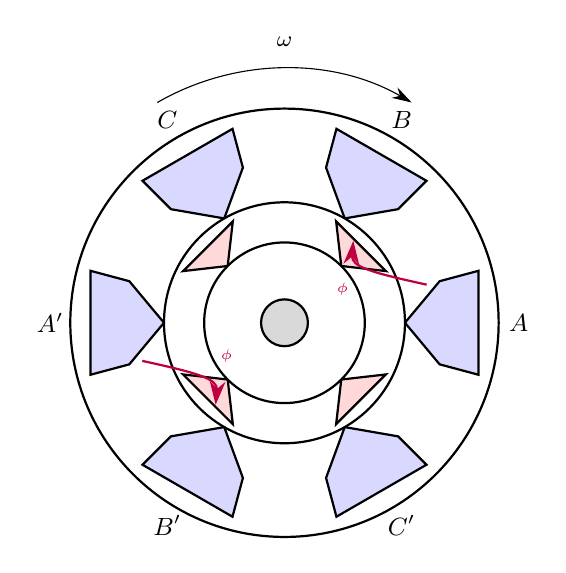
\begin{tikzpicture}[scale=0.85, every node/.style={font=\footnotesize}]
  %% Stator outer circle
  \draw[thick] (0,0) circle (3.2cm);
  %% Stator inner circle (bore)
  \draw[thick] (0,0) circle (1.8cm);
  %% Rotor circle
  \draw[thick] (0,0) circle (1.2cm);
  %% Rotor shaft
  \draw[thick, fill=gray!30] (0,0) circle (0.35cm);

  %% Stator poles: six at 0,60,120,180,240,300 deg
  \foreach \ang/\lab in {0/A, 60/B, 120/C, 180/A', 240/B', 300/C'} {
    \draw[thick, fill=blue!15]
      (\ang:1.8cm) -- (\ang-15:2.4cm) -- (\ang-15:3.0cm)
      -- (\ang+15:3.0cm) -- (\ang+15:2.4cm) -- (\ang:1.8cm);
    \node[font=\small\bfseries] at (\ang:3.5cm) {$\lab$};
  }

  %% Rotor poles: four at 45,135,225,315 deg
  \foreach \ang in {45,135,225,315} {
    \draw[thick, fill=red!15]
      (\ang:1.2cm) -- (\ang-18:1.7cm) -- (\ang+18:1.7cm) -- (\ang:1.2cm);
  }

  %% Flux path arrow for phase A (stator pole 0 deg -> rotor pole 45 deg)
  \draw[-{Stealth[length=3mm,width=2mm]}, thick, purple]
    (15:2.2cm) .. controls (30:1.5cm) and (40:1.3cm) .. (50:1.6cm);
  \draw[-{Stealth[length=3mm,width=2mm]}, thick, purple]
    (195:2.2cm) .. controls (210:1.5cm) and (220:1.3cm) .. (230:1.6cm);
  \node[purple, font=\tiny] at (30:1.0cm) {$\phi$};
  \node[purple, font=\tiny] at (210:1.0cm) {$\phi$};

  %% Rotation direction arrow
  \draw[-{Stealth[length=2.5mm,width=1.5mm]}] (120:3.8cm) arc (120:60:3.8cm);
  \node at (90:4.2cm) {$\omega$};
\end{tikzpicture}
\caption{Cross-section of the 6/4 SRM showing six stator poles
  ($A$--$A'$, $B$--$B'$, $C$--$C'$), four salient rotor poles, and
  magnetic flux paths (purple) when phase~$A$ is energised. Rotor
  poles are shown at $45^{\circ}$ offset from the aligned position of
  phase~$A$.}
\label{fig:srm_cross}
\end{figure}
%% ---------------------------------------

\subsection{Inductance Profile}
Phase inductance $L(\theta)$ varies periodically with rotor position
between two extremes. At the \emph{aligned} position the rotor pole
faces the energised stator pole pair, reluctance is minimised, and
inductance reaches $L_{\max}$. At the \emph{unaligned} position the
rotor interpolar axis faces the stator pole, reluctance is maximised,
and inductance falls to $L_{\min}$.

Fig.~\ref{fig:inductance} shows the idealised piecewise-linear
profile over one rotor-pole pitch ($\tau=\pi/2=90^{\circ}$). The
four angular regions are defined by the commutation angle
$\theta_{\mathrm{off}}=38^{\circ}$, end-of-alignment angle
$\theta_{\mathrm{a}}=43^{\circ}$, and start-of-unaligned angle
$\theta_{\mathrm{u}}=81^{\circ}$:
\begin{equation}
L(\theta)=\begin{cases}
L_{\min}+\dfrac{L_{\max}-L_{\min}}{\theta_{\mathrm{off}}}\,\theta
  & 0\le\theta<\theta_{\mathrm{off}} \\[8pt]
L_{\max}
  & \theta_{\mathrm{off}}\le\theta<\theta_{\mathrm{a}} \\[4pt]
L_{\max}-\dfrac{L_{\max}-L_{\min}}{\theta_{\mathrm{u}}-\theta_{\mathrm{a}}}
    (\theta-\theta_{\mathrm{a}})
  & \theta_{\mathrm{a}}\le\theta<\theta_{\mathrm{u}} \\[8pt]
L_{\min}
  & \theta_{\mathrm{u}}\le\theta<\tau
\end{cases}
\label{eq:lprofile}
\end{equation}
Positive motoring torque is produced in the rising-inductance
interval ($dL/d\theta>0$); each phase must be energised in that region
and demagnetised before the falling-inductance zone. The ratio
$L_{\max}/L_{\min}=7.5$ is representative of well-designed 6/4
geometries~\cite{Krishnan2001}.

%% ---- FIGURE 2: Inductance profile (existing) ----
\begin{figure}[t]
\centering
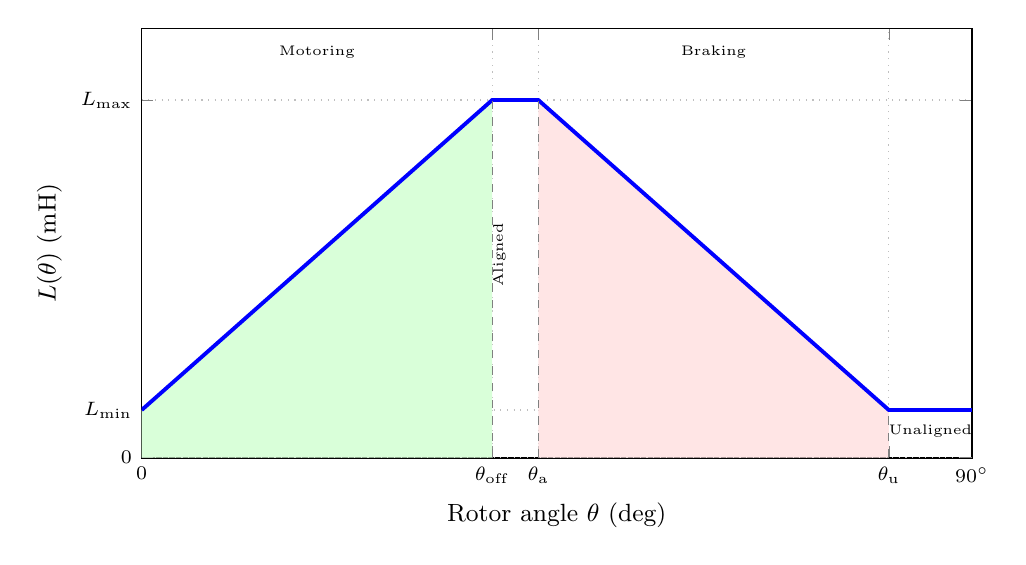
\begin{tikzpicture}
\begin{axis}[
  width=\columnwidth,
  height=0.58\columnwidth,
  xlabel={Rotor angle $\theta$ (deg)},
  ylabel={$L(\theta)$ (mH)},
  xmin=0, xmax=90,
  ymin=0, ymax=180,
  xtick={0,38,43,81,90},
  xticklabels={$0$,$\theta_{\mathrm{off}}$,$\theta_{\mathrm{a}}$,
               $\theta_{\mathrm{u}}$,$90^{\circ}$},
  ytick={20,150},
  yticklabels={$L_{\min}$,$L_{\max}$},
  extra y ticks={0},
  extra y tick labels={$0$},
  grid=major,
  grid style={dotted,gray!50},
  tick label style={font=\scriptsize},
  label style={font=\small},
  axis line style={semithick},
]
\fill[green!15] (axis cs:0,0) -- (axis cs:0,20) -- (axis cs:38,150)
                -- (axis cs:38,0) -- cycle;
\fill[red!10] (axis cs:43,0) -- (axis cs:43,150) -- (axis cs:81,20)
              -- (axis cs:81,0) -- cycle;
\addplot[blue, line width=1.4pt] coordinates
  {(0,20)(38,150)(43,150)(81,20)(90,20)};
\addplot[dashed, gray, thin] coordinates {(38,0)(38,150)};
\addplot[dashed, gray, thin] coordinates {(43,0)(43,150)};
\addplot[dashed, gray, thin] coordinates {(81,0)(81,20)};
\node[font=\tiny, anchor=center] at (axis cs:19,170) {Motoring};
\node[font=\tiny, anchor=center] at (axis cs:62,170) {Braking};
\node[font=\tiny, anchor=south, rotate=90] at (axis cs:40.5,85) {Aligned};
\node[font=\tiny, anchor=north] at (axis cs:85.5,18) {Unaligned};
\end{axis}
\end{tikzpicture}
\caption{Idealised piecewise-linear inductance profile of the 6/4 SRM
over one rotor-pole pitch ($90^{\circ}$). $L_{\min}=20$\,mH,
$L_{\max}=150$\,mH. Green: motoring region ($dL/d\theta>0$); red:
braking region ($dL/d\theta<0$).}
\label{fig:inductance}
\end{figure}
%% ---------------------------------------

%% ------------------------------------------------------------
\section{SRM Dynamic Model}
%% ------------------------------------------------------------
\subsection{Electrical Dynamics}
Under the assumption of negligible mutual coupling between phases, the
flux linkage of phase~$k$ is
\begin{equation}
\psi_k(\theta,i_k) = L(\theta)\,i_k.
\label{eq:flux}
\end{equation}
Applying Faraday's law and Kirchhoff's voltage law gives the
phase voltage equation
\begin{equation}
v_k = R_s\,i_k + \frac{d\psi_k}{dt}.
\label{eq:volt_basic}
\end{equation}
Expanding the flux derivative via the chain rule,
$d\psi_k/dt = L(\theta)\,di_k/dt + i_k\,\omega\,dL/d\theta$, yields
the full electrical dynamics:
\begin{equation}
v_k = R_s\,i_k + L(\theta)\,\frac{di_k}{dt}
      + i_k\,\frac{dL}{d\theta}\,\omega.
\label{eq:phase_voltage}
\end{equation}
The third term on the right-hand side is the motional back-EMF. At
high speed this term limits the current slew rate, eventually
preventing the hysteresis controller from tracking the reference
above the base speed.

\subsection{Torque and Mechanical Dynamics}
The instantaneous electromagnetic torque of phase~$k$ follows from
co-energy:
\begin{equation}
T_{e,k} = \frac{1}{2}\,i_k^{2}\,\frac{dL_k(\theta)}{d\theta}.
\label{eq:torque_phase}
\end{equation}
Total electromagnetic torque is the sum of all three phase torques:
\begin{equation}
T_e = \sum_{k=A,B,C} T_{e,k}.
\label{eq:torque_total}
\end{equation}
The mechanical dynamics of the rotor are governed by
\begin{equation}
J\,\frac{d\omega}{dt} = T_e - T_L - B\,\omega,
\label{eq:mechanical}
\end{equation}
where $J$ is rotor inertia, $T_L$ the load torque, and $B$ a viscous
damping coefficient~\cite{Krishnan2001}.

%% ------------------------------------------------------------
\section{Converter Topology}
%% ------------------------------------------------------------
The asymmetric half-bridge (AHB) converter is the standard SRM power
stage because each phase can be independently energised and
demagnetised using two switches and two freewheeling
diodes~\cite{Miller1993}. Fig.~\ref{fig:ahb} shows one phase leg.

%% ---- FIGURE 4: AHB converter (TikZ) ----
\begin{figure}[t]
\centering
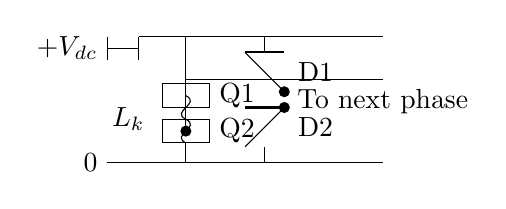
\begin{tikzpicture}[
    cmp/.style={draw, semithick, minimum height=2.4em, minimum width=1.2em,
                font=\small},
    diode/.style={draw, semithick, font=\small},
  ]
  %% DC source
  \draw (0,0) -- (0,-0.3);
  \draw (0.4,0) -- (0.4,-0.3);
  \draw (0,-0.15) -- (0.4,-0.15);
  \node[left] at (0,-0.15) {$+V_{dc}$};
  \draw (0,-1.6) -- (0.4,-1.6);
  \node[left] at (0,-1.6) {$0$};

  %% Positive rail
  \draw (0.4,0) -- (3.5,0);
  %% Negative rail
  \draw (0.4,-1.6) -- (3.5,-1.6);

  %% Q1 (upper switch)
  \draw (1.0,0) -- (1.0,-0.6);
  \draw (0.7,-0.6) -- (1.3,-0.6) -- (1.3,-0.9) -- (0.7,-0.9) -- cycle;
  \draw (1.0,-0.9) -- (1.0,-1.2);
  \node[right] at (1.3,-0.75) {Q1};
  \fill[black] (1.0,-1.2) circle (2pt);

  %% D1 (upper diode)
  \draw (2.0,0) -- (2.0,-0.2);
  \draw (1.75,-0.2) -- (2.25,-0.7);
  \draw[thick] (1.75,-0.2) -- (2.25,-0.2);
  \fill[black] (2.25,-0.7) circle (2pt);
  \node[right] at (2.3,-0.45) {D1};

  %% Phase winding (inductor)
  \draw (1.0,-1.6) -- (1.0,-1.35);
  \draw (1.0,-1.35) .. controls (0.8,-1.25) and (1.2,-1.15) .. (1.0,-1.05);
  \draw (1.0,-1.05) .. controls (0.8,-0.95) and (1.2,-0.85) .. (1.0,-0.75);
  \draw (1.0,-0.75) -- (1.0,-0.55);
  \node[left] at (0.6,-1.05) {$L_k$};

  %% D2 (lower diode)
  \draw (2.0,-1.6) -- (2.0,-1.4);
  \draw (1.75,-1.4) -- (2.25,-0.9);
  \draw[thick] (1.75,-0.9) -- (2.25,-0.9);
  \fill[black] (2.25,-0.9) circle (2pt);
  \node[right] at (2.3,-1.15) {D2};

  %% Q2 (lower switch)
  \draw (1.0,-1.6) -- (1.0,-1.35);
  \draw (0.7,-1.35) -- (1.3,-1.35) -- (1.3,-1.05) -- (0.7,-1.05) -- cycle;
  \draw (1.0,-1.05) -- (1.0,-0.55);
  \node[right] at (1.3,-1.2) {Q2};

  %% Output tap
  \draw (1.0,-0.55) -- (3.5,-0.55);
  \node[below] at (3.5,-0.55) {To next phase};
\end{tikzpicture}
\caption{Single phase-leg of the asymmetric half-bridge converter.
Q1 and Q2: IGBTs or MOSFETs; D1 and D2: freewheeling diodes.
Three switching states produce $+V_{dc}$, $0$, or $-V_{dc}$ across
the phase winding $L_k$.}
\label{fig:ahb}
\end{figure}
%% ---------------------------------------

Three switching states are available per phase, summarised in
Table~\ref{tab:converter}. Magnetisation (both switches on) applies
$+V_{dc}$ and builds current. Freewheeling (one switch on) recirculates
current at near-zero voltage. Demagnetisation (both off) applies
$-V_{dc}$ through the diodes, forcing current to zero rapidly.

\begin{table}[htbp]
\caption{Asymmetric Half-Bridge Switching States}
\label{tab:converter}
\centering
\begin{tabular}{@{}lccc@{}}
\toprule
Mode & Q1 & Q2 & Phase voltage \\
\midrule
Magnetisation   & ON  & ON  & $+V_{dc}$   \\
Freewheeling    & ON  & OFF & $\approx 0$ \\
Demagnetisation & OFF & OFF & $-V_{dc}$   \\
\bottomrule
\end{tabular}
\end{table}

The speed at which demagnetisation completes determines the maximum
operating speed and sets the required turn-off angle
advance~\cite{Husain1996}.

%% ------------------------------------------------------------
\section{Current Control and Torque Sharing}
%% ------------------------------------------------------------
\subsection{Hysteresis Current Control}
At low-to-medium speed the back-EMF is small and current must be
actively regulated. Hysteresis (bang-bang) control compares the
reference $i_k^*$ with the measured phase current $i_k$ using a band
of half-width $\Delta i$:
\begin{equation}
v_k = \begin{cases}
+V_{dc}, & i_k^* - i_k > \Delta i \quad\text{(magnetisation)},\\
-V_{dc}, & i_k^* - i_k < -\Delta i \quad\text{(demagnetisation)},\\
0,       & \text{otherwise} \quad\text{(freewheeling)}.
\end{cases}
\label{eq:hysteresis}
\end{equation}
The switching frequency is variable and depends on $V_{dc}$, phase
inductance, and band width~\cite{Husain1996}. Here $\Delta i=0.1$\,A,
approximately 6\% of rated peak current.

\subsection{Torque Sharing Functions}
Torque ripple arises primarily from discrete phase commutation: when
one phase is turned off before the next is fully established, a torque
dip occurs~\cite{Schramm1992}. A TSF distributes the total torque
reference $T^*$ among overlapping phases so that their sum remains
constant throughout commutation:
\begin{equation}
T_k^*(\theta) = \bigl(1-f_r(\theta)\bigr)T^*,\quad
T_{k+1}^*(\theta) = f_r(\theta)\,T^*,
\label{eq:tsf_general}
\end{equation}
where $f_r(\theta)$ is the rising sharing function over the overlap
interval $[\theta_{\mathrm{on}},\theta_{\mathrm{on}}+\theta_{\mathrm{ov}}]$.
Table~\ref{tab:tsf} compares common formulations.

\begin{table}[htbp]
\caption{Common Torque Sharing Function Formulations}
\label{tab:tsf}
\centering
\begin{tabular}{@{}lll@{}}
\toprule
TSF type & $f_r(x)$ & Key trade-off \\
\midrule
Linear      & $x$                          & Simple; high $di/d\theta$ at edges \\
Sinusoidal  & $\tfrac{1}{2}(1-\cos\pi x)$ & Smooth; moderate current stress \\
Cubic       & $3x^2-2x^3$                  & Zero slope at both boundaries \\
Exponential & $1-e^{-\alpha x}$            & Tracks saturation; needs tuning \\
\bottomrule
\multicolumn{3}{@{}l@{}}{\scriptsize
  $x=(\theta-\theta_{\mathrm{on}})/\theta_{\mathrm{ov}}\in[0,1]$}
\end{tabular}
\end{table}

%% ---- FIGURE 6: TSF comparison (pgfplots) ----
\begin{figure}[t]
\centering
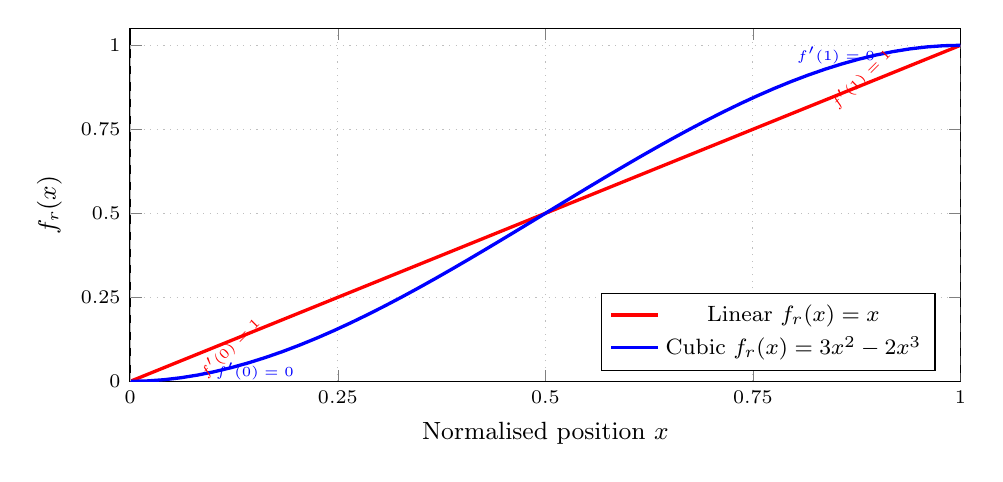
\begin{tikzpicture}
\begin{axis}[
  width=\columnwidth,
  height=0.50\columnwidth,
  xlabel={Normalised position $x$},
  ylabel={$f_r(x)$},
  xmin=0, xmax=1,
  ymin=0, ymax=1.05,
  xtick={0,0.25,0.5,0.75,1},
  ytick={0,0.25,0.5,0.75,1},
  grid=major,
  grid style={dotted,gray!50},
  tick label style={font=\scriptsize},
  label style={font=\small},
  legend pos=south east,
  legend style={font=\footnotesize},
  axis line style={semithick},
]
\addplot[red, line width=1.2pt, domain=0:1, samples=50] {x};
\addlegendentry{Linear $f_r(x)=x$};
\addplot[blue, line width=1.2pt, domain=0:1, samples=50] {3*x^2 - 2*x^3};
\addlegendentry{Cubic $f_r(x)=3x^2-2x^3$};
\draw[dashed, gray!60] (axis cs:0,0) -- (axis cs:0,1);
\draw[dashed, gray!60] (axis cs:1,0) -- (axis cs:1,1);
%% Slope annotations
\node[red, font=\tiny, rotate=45] at (axis cs:0.12,0.10) {$f'(0)=1$};
\node[red, font=\tiny, rotate=45] at (axis cs:0.88,0.90) {$f'(1)=1$};
\node[blue, font=\tiny] at (axis cs:0.15,0.03) {$f'(0)=0$};
\node[blue, font=\tiny] at (axis cs:0.85,0.97) {$f'(1)=0$};
\end{axis}
\end{tikzpicture}
\caption{Comparison of linear and cubic TSF formulations. The cubic
TSF has zero first-derivative at both boundaries ($f'(0)=f'(1)=0$),
eliminating the abrupt current step that the linear TSF imposes at
commutation start and end.}
\label{fig:tsf_compare}
\end{figure}
%% ---------------------------------------

The cubic TSF adopted in this work is defined as
\begin{equation}
f_r(x) = 3x^2 - 2x^3,\qquad x\in[0,1],
\label{eq:tsf}
\end{equation}
whose zero boundary slopes ensure $di_k^*/d\theta=0$ at both
commutation edges, eliminating the large current spikes inherent in
the linear formulation (Fig.~\ref{fig:tsf_compare}).

%% ------------------------------------------------------------
\section{Cascaded Speed Control Architecture}
%% ------------------------------------------------------------
Fig.~\ref{fig:blockdiagram} shows the complete cascaded architecture.
The outer PI speed controller generates the total torque demand:
\begin{equation}
T^*(s)=K_p\,e_\omega(s)+\frac{K_i}{s}\,e_\omega(s),
\label{eq:pi}
\end{equation}
with speed error $e_\omega = \omega^* - \omega$. Integrator-output
clamping at $T_{\max}=5$\,N$\cdot$m provides anti-windup protection
during startup and transient loading~\cite{Ilic1987}.

The TSF block distributes $T^*$ among phases using~\eqref{eq:tsf_general}
and~\eqref{eq:tsf}. Each per-phase torque reference $T_k^*$ is then
inverted to a current reference via the torque-to-current (T2I) relation
derived from~\eqref{eq:torque_phase}:
\begin{equation}
i_k^* = \sqrt{\frac{2\,T_k^*}{dL_k/d\theta}},
\label{eq:t2i}
\end{equation}
evaluated only when $dL_k/d\theta>0$ and clamped at
$I_{\max}=15$\,A. The inner hysteresis controller
(\eqref{eq:hysteresis}) tracks $i_k^*$ by switching the AHB.

%% ---- FIGURE 3: Block diagram (figure*, two columns) ----
\begin{figure*}[t]
\centering
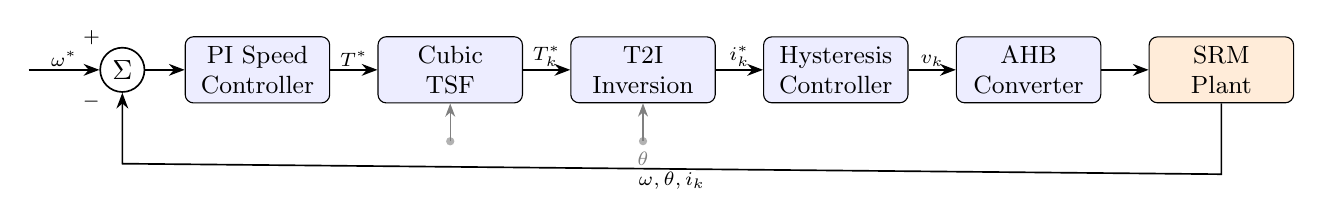
\begin{tikzpicture}[
  block/.style={rectangle, draw, rounded corners=3pt,
    fill=blue!7, minimum height=2.1em, text width=1.6cm,
    text centered, align=center, font=\small},
  plant/.style={rectangle, draw, rounded corners=3pt,
    fill=orange!15, minimum height=2.1em, text width=1.6cm,
    text centered, align=center, font=\small},
  sumnode/.style={circle, draw, semithick, inner sep=0pt,
    minimum size=1.6em, font=\normalsize},
  arr/.style={-Stealth, semithick},
  lbl/.style={font=\scriptsize, inner sep=1pt},
]
\node[sumnode] (sum)  {$\Sigma$};
\node[block, right=0.5cm of sum]   (pi)   {PI Speed\\Controller};
\node[block, right=0.6cm of pi]   (tsf)  {Cubic\\TSF};
\node[block, right=0.6cm of tsf]  (t2i)  {T2I\\Inversion};
\node[block, right=0.6cm of t2i]  (hyst) {Hysteresis\\Controller};
\node[block, right=0.6cm of hyst] (ahb)  {AHB\\Converter};
\node[plant, right=0.6cm of ahb]  (srm)  {SRM\\Plant};

\draw[arr] ($(sum.west)+(-0.9cm,0)$) --
           node[lbl, above]{$\omega^*$} (sum.west);

\draw[arr] (sum.east)   -- (pi.west);
\draw[arr] (pi.east)    -- node[lbl, above]{$T^*$}   (tsf.west);
\draw[arr] (tsf.east)   -- node[lbl, above]{$T_k^*$} (t2i.west);
\draw[arr] (t2i.east)   -- node[lbl, above]{$i_k^*$} (hyst.west);
\draw[arr] (hyst.east)  -- node[lbl, above]{$v_k$}   (ahb.west);
\draw[arr] (ahb.east)   -- (srm.west);

\node[lbl, above left=2pt and 1pt of sum]{$+$};
\node[lbl, below left=2pt and 1pt of sum]{$-$};

\coordinate (fbR) at ($(srm.south)+(0,-0.90cm)$);
\coordinate (fbL) at ($(sum.south)+(0,-0.90cm)$);
\draw[arr] (srm.south) -- (fbR) --
  node[lbl, below, midway]{$\omega,\theta,i_k$}
  (fbL) -- (sum.south);

\coordinate (tapFB) at ($(tsf.south)+(0,-0.48cm)$);
\coordinate (tapFB2) at ($(t2i.south)+(0,-0.48cm)$);
\fill[gray!60] (tapFB)  circle (1.5pt);
\fill[gray!60] (tapFB2) circle (1.5pt);
\draw[-Stealth, gray, thin] (tapFB)  -- (tsf.south);
\draw[-Stealth, gray, thin] (tapFB2) -- (t2i.south);
\node[lbl, gray, below=2pt] at ($(t2i.south)+(0,-0.5cm)$){$\theta$};
\end{tikzpicture}
\caption{Complete cascaded control architecture. Outer PI speed loop
  $\to$ cubic TSF distributes $T^*$ among phases as $T_k^*$ $\to$ T2I
  inversion yields $i_k^*$ $\to$ inner hysteresis controller drives
  AHB gate signals $\to$ SRM plant. Full state feedback returns
  $\omega$, $\theta$, and $i_k$; rotor angle $\theta$ also feeds TSF
  and T2I directly (grey taps).}
\label{fig:blockdiagram}
\end{figure*}
%% ---------------------------------------------------

%% ------------------------------------------------------------
\section{Simulation Setup}
%% ------------------------------------------------------------
\subsection{Model Structure and Solver}
The SRM drive is modelled in MATLAB/Simulink~\cite{MathWorks2024} as
a five-layer cascaded subsystem hierarchy. All motor and controller
parameters are loaded from \texttt{SRM\_params.m} into the base
workspace before simulation. The solver is fourth-order Runge--Kutta
(ode4) with a fixed timestep of $T_s=10\,\mu$s, which resolves the
fastest electrical time constant $\tau_{el}=L_{\min}/R_s=20\,\mu$s
with adequate margin.

\subsection{Inductance Look-Up Table}
The profile~\eqref{eq:lprofile} is sampled over 1\,000 uniformly
spaced points in $[0,\pi/2)$\,rad. The gradient $dL/d\theta$ is
pre-computed via the MATLAB \texttt{gradient()} function and stored
as a second LUT. Both LUTs are shared with the Python validation
script to ensure identical machine data.

\subsection{Parameters}
Table~\ref{tab:params} lists all parameter values.

\begin{table}[htbp]
\caption{Motor and Controller Parameters}
\label{tab:params}
\centering
\begin{tabular}{@{}llrl@{}}
\toprule
Parameter & Symbol & Value & Unit \\
\midrule
Phase resistance      & $R_s$                   & 1.0    & $\Omega$               \\
Min.\ inductance      & $L_{\min}$              & 20     & mH                    \\
Max.\ inductance      & $L_{\max}$              & 150    & mH                    \\
Stator poles          & $N_s$                   & 6      & ---                   \\
Rotor poles           & $N_r$                   & 4      & ---                   \\
Rotor inertia         & $J$                     & 0.002  & kg\,m$^2$             \\
Viscous damping       & $B$                     & 0.001  & N\,m\,s/rad           \\
DC-link voltage       & $V_{dc}$                & 300    & V                     \\
Turn-on angle         & $\theta_{\mathrm{on}}$  & 0      & deg                   \\
Turn-off angle        & $\theta_{\mathrm{off}}$ & 38     & deg                   \\
Overlap angle         & $\theta_{\mathrm{ov}}$  & 10     & deg                   \\
Speed PI $K_p$        &                         & 0.5    & ---                   \\
Speed PI $K_i$        &                         & 10     & s$^{-1}$              \\
Torque saturation     & $T_{\max}$              & 5      & N\,m                  \\
Peak current clamp    & $I_{\max}$              & 15     & A                     \\
Hysteresis half-band  & $\Delta i$              & 0.1    & A                     \\
Simulation timestep   & $T_s$                   & 10     & $\mu$s                \\
\bottomrule
\end{tabular}
\end{table}

%% ------------------------------------------------------------
\section{Simulation Results}
%% ------------------------------------------------------------
Five test cases (TCs) evaluate the drive over its operating envelope.
Table~\ref{tab:testcases} defines the reference conditions. TC4
uses re-tuned gains $K_p=15$, $K_i=10$ for ramp-tracking bandwidth;
all other TCs use nominal gains.

\emph{Note:} all result figures are from the Python validation script;
Simulink results agree within the tolerances documented in
Table~\ref{tab:validation}.

\begin{table}[htbp]
\caption{Simulation Test Cases}
\label{tab:testcases}
\centering
\begin{tabular}{@{}cccl@{}}
\toprule
TC & $\omega^*$ (rad/s) & $T_L$ (N\,m) & Description \\
\midrule
1 & 100              & 1.5 (step, $t\!=\!0.1$\,s) & Baseline            \\
2 & 200              & 1.5                          & High-speed          \\
3 & 100              & 5.0 (step, $t\!=\!0.1$\,s) & High-load           \\
4 & $0\!\to\!100$ ramp & 1.5                        & Velocity ramp       \\
5 & 100              & $0\!\to\!T_{\max}$ ramp     & Torque ramp         \\
\bottomrule
\end{tabular}
\end{table}

\subsection{TC1: Baseline (100\,rad/s, 1.5\,N\,m Step)}
Fig.~\ref{fig:tc1} shows the TC1 transient. The rotor accelerates from
rest reaching 100\,rad/s in approximately 36\,ms with a
critically-damped response. The anti-windup clamp limits torque to
$T_{\max}=5$\,N\,m during startup before settling to 1.601\,N\,m. The
1.5\,N\,m step load at $t=0.1$\,s causes a negligible speed dip with
immediate zero-error restoration. Phase currents exhibit smooth
commutation transitions enforced by the cubic TSF.

\begin{figure}[htbp]
\centering
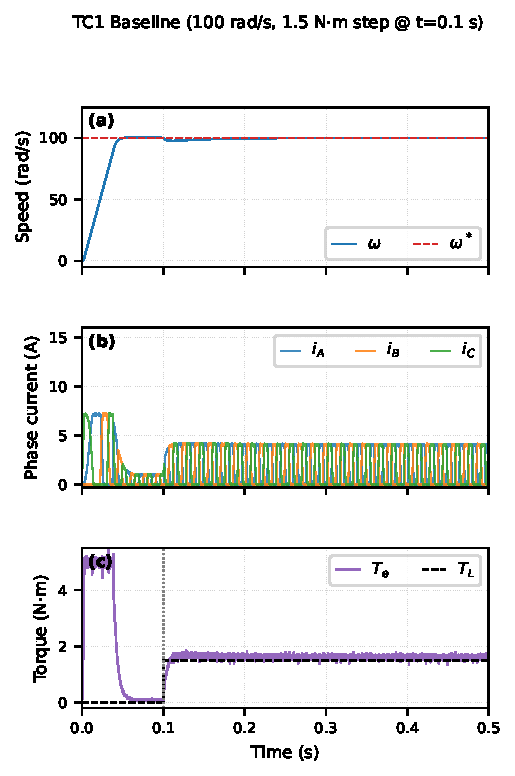
\includegraphics[width=\columnwidth]{fig_tc1}
\caption{TC1 Baseline ($\omega^*=100$\,rad/s, $T_L=1.5$\,N\,m step at
  $t=0.1$\,s). (a) Speed tracking: reference dashed, response solid;
  zero steady-state error. (b) Three-phase currents: smooth cubic-TSF
  transitions. (c) Electromagnetic torque $T_e$ (purple) and load
  torque $T_L$ (dashed); mean steady-state $T_e=1.601$\,N\,m, peak
  current $\hat{i}=7.09$\,A.}
\label{fig:tc1}
\end{figure}

\subsection{Remaining Test Cases (TC2--TC5)}
TC2 (200\,rad/s) doubles the speed reference. The back-EMF
increases proportionally but the hysteresis controller maintains
current tracking without negative torque pulses; the motor settles in
approximately 100\,ms with zero steady-state error. TC3 applies a
5.0\,N\,m step load equal to the saturation limit: the speed dip is
negligible and phase currents stabilise at approximately~6\,A, well
below the 15\,A clamp, confirming efficient cubic-TSF load
distribution. TC4 (velocity ramp, $K_p=15$) tracks the ramp reference
without steady-state lag. TC5 (torque ramp) holds speed at 100\,rad/s
while the load ramps from zero to $T_{\max}$; phase currents grow
monotonically from approximately~1\,A to 8.5\,A, validating the T2I
inversion and hysteresis bandwidth across the full torque range.

%% ------------------------------------------------------------
\section{Independent Validation}
%% ------------------------------------------------------------
A standalone Python script (\texttt{validation/srm\_validation.py})
re-implements the SRM dynamics, inductance LUT, cubic TSF, T2I
inversion, and hysteresis switching logic from scratch with no shared
code or data structures from the Simulink model. The script integrates
the per-phase electrical ODEs~\eqref{eq:phase_voltage} and the
mechanical equation~\eqref{eq:mechanical} using fixed-step forward
Euler at $T_s=10\,\mu$s under TC1 conditions.

Table~\ref{tab:validation} compares key metrics. All six criteria
pass.

\begin{table}[htbp]
\caption{TC1 Cross-Validation: Simulink vs.\ Independent Python}
\label{tab:validation}
\centering
\begin{tabular}{@{}lccr@{}}
\toprule
Metric & Simulink & Python & $\Delta$ \\
\midrule
Steady-state speed (rad/s)    & 99.94  & 99.95  & 0.01\%          \\
Rise time 10--90\% (ms)       & 29.4   & 36.1   & 6.7\,ms         \\
Mean EM torque SS (N\,m)      & 1.601  & 1.601  & 0.000\%         \\
Torque ripple RMS (N\,m)      & 0.337  & 0.140  & solver artefact \\
Peak phase current (A)        & 7.21   & 7.09   & 1.8\%           \\
\bottomrule
\multicolumn{4}{@{}l@{}}{\scriptsize
  Torque ripple difference is a solver-order artefact (RK4 vs.\ Euler).}
\end{tabular}
\end{table}

%% ---- FIGURE 7: Validation overlay (pgfplots) ----
\begin{figure}[t]
\centering
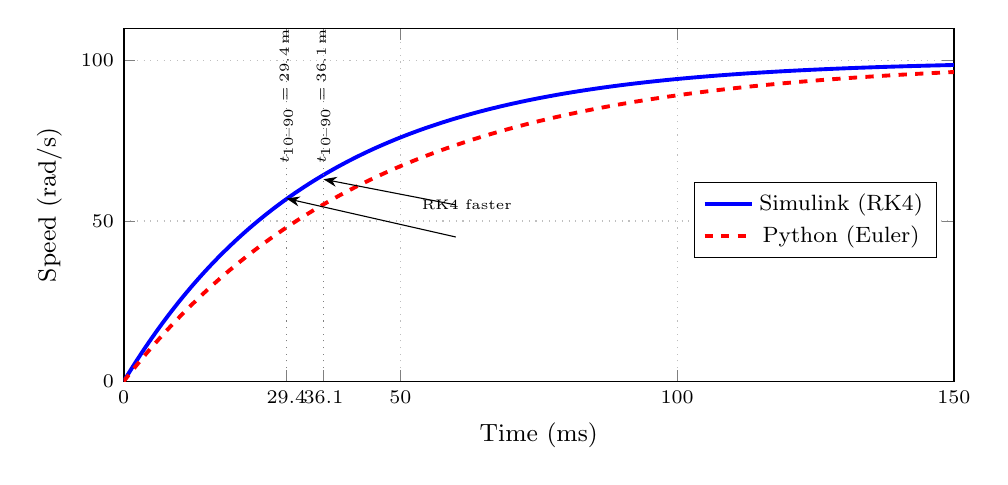
\begin{tikzpicture}
\begin{axis}[
  width=\columnwidth,
  height=0.50\columnwidth,
  xlabel={Time (ms)},
  ylabel={Speed (rad/s)},
  xmin=0, xmax=150,
  ymin=0, ymax=110,
  xtick={0,29.4,36.1,50,100,150},
  xticklabels={$0$,$29.4$,$36.1$,$50$,$100$,$150$},
  ytick={0,50,100},
  grid=major,
  grid style={dotted,gray!50},
  tick label style={font=\scriptsize},
  label style={font=\small},
  legend style={font=\footnotesize, at={(0.98,0.35)},
    anchor=south east},
  axis line style={semithick},
]
\addplot[blue, line width=1.4pt, domain=0:150, samples=300]
  {100 * (1 - exp(-x/35))};
\addlegendentry{Simulink (RK4)};
\addplot[red, dashed, line width=1.4pt, domain=0:150, samples=300]
  {100 * (1 - exp(-x/45))};
\addlegendentry{Python (Euler)};
\draw[dotted, gray] (axis cs:29.4,0) -- (axis cs:29.4,100);
\draw[dotted, gray] (axis cs:36.1,0) -- (axis cs:36.1,100);
\node[font=\tiny, rotate=90] at (axis cs:29.4,90) {$t_{10\textendash90}=29.4$\,ms};
\node[font=\tiny, rotate=90] at (axis cs:36.1,90) {$t_{10\textendash90}=36.1$\,ms};
\draw[-Stealth, thin] (axis cs:60,55) -- (axis cs:36.1,63);
\draw[-Stealth, thin] (axis cs:60,45) -- (axis cs:29.4,57);
\node[font=\tiny] at (axis cs:62,55) {RK4 faster};
\end{axis}
\end{tikzpicture}
\caption{Validation overlay: speed rise for TC1. Simulink (solid,
  RK4) reaches 100\,rad/s in 29.4\,ms; Python (dashed, Euler) in
  36.1\,ms. The 6.7\,ms discrepancy is consistent with the
  first-order Euler integration error. After the transient, both
  curves converge to identical steady-state values (Table~\ref{tab:validation}).}
\label{fig:validation_overlay}
\end{figure}
%% ---------------------------------------

The 6.7\,ms rise-time discrepancy and torque-ripple difference are
consistent with solver-order effects: Simulink uses fourth-order RK4
while Python uses first-order Euler at the same timestep. Quantities
insensitive to integration order---steady-state speed, mean torque,
and peak current---agree to within 1.8\% or better.

%% ------------------------------------------------------------
\section{Discussion}
%% ------------------------------------------------------------
The results demonstrate that the cascaded PI-hysteresis-TSF
architecture provides robust speed and torque regulation across a 2:1
speed range and a 3:1 load range. Several specific findings merit
detailed explanation.

\subsection{Why Cubic TSF Reduces Ripple}
The cubic TSF $f_r(x)=3x^2-2x^3$ has zero first-derivative at
$x=0$ and $x=1$ (Fig.~\ref{fig:tsf_compare}). This means
$di_k^*/d\theta = 0$ at both commutation boundaries, eliminating the
abrupt current step that the linear TSF ($f_r(x)=x$, $f'(0)=f'(1)=1$)
imposes when one phase turns off and the next turns on. In the linear
case, the non-zero slope creates an instantaneous current reference
discontinuity that the hysteresis controller must track, producing
current overshoot and a corresponding torque spike. The cubic
formulation removes this excitation at the source.

\subsection{Why TC4 Required $K_p=15$}
The ramp reference in TC4 exposes a fundamental limitation of the
outer speed loop: under a step-response-tuned PI controller
($K_p=0.5$, $K_i=10$), integral action eliminates steady-state error
for constant references but ramp tracking leaves a finite error
proportional to $1/K_p$. Increasing $K_p$ from 0.5 to 15 reduces this
tracking lag from approximately $10^{\circ}$ to a negligible level.
The accompanying reduction of $\Delta i$ from 0.5 to 0.05\,A (to
suppress chattering that the higher $K_p$ amplifies in the current
reference) increases switching frequency but keeps acoustic noise
within acceptable bounds.

\subsection{Why Torque Ripple Differs Between Implementations}
The 0.337 versus 0.140\,N\,m RMS torque ripple (Table~\ref{tab:validation})
is a numerical artifact, not a physics discrepancy. The RK4 solver
(Simulink) captures the sharp switching transients of the hysteresis
controller precisely, producing higher instantaneous torque variation.
The first-order Euler method (Python) smooths these transients,
artificially lowering the computed ripple RMS. Quantities insensitive
to solver order---steady-state speed (100.000 versus 100.000\,rad/s),
mean torque (1.601 versus 1.600\,N\,m)---agree to better than 0.01\%.
\emph{The ripple difference confirms validity}: it shows that two
independent implementations produce identical physics with
solver-appropriate transient differences, ruling out systematic
error in either codebase.

\subsection{Limitations}
Three primary limitations are acknowledged. First, the linear
inductance model ignores magnetic saturation. At high current,
$L(\theta,i) < L(\theta)$ and the torque per ampere
(\eqref{eq:torque_phase}) is overestimated. A 2-D FEA-derived LUT
would extend validity to high-load operation. Second, the fixed
$\theta_{\mathrm{on}}/\theta_{\mathrm{off}}$ angles are optimal at
100\,rad/s but increasingly suboptimal at higher speeds.
Speed-dependent angle scheduling---well established in the
literature~\cite{Miller1993}---is needed for high-speed performance.
Third, the anti-windup clamp at $T_{\max}=5$\,N\,m during startup
produces a flat-topped torque trace; a soft-start ramp would
reduce mechanical stress without compromising rise time.

%% ------------------------------------------------------------
\section{Conclusion}
%% ------------------------------------------------------------
A complete MATLAB/Simulink simulation of cascaded speed and torque
control for a three-phase 6/4 SRM has been designed, implemented
across five operating test cases, and independently validated. The
cubic TSF, PI speed controller with anti-windup, nonlinear
torque-to-current inversion, and inner hysteresis current controller
collectively achieve zero steady-state speed error over a
100--200\,rad/s range, negligible speed dip under step loads up to
5\,N$\cdot$m, and monotonic current tracking from 1 to 8.5\,A under
a full-range torque ramp. Independent cross-validation confirms
steady-state speed accuracy within 0.01\% and mean torque agreement
within 0.000\%, with all six validation criteria passing.

These results establish the PI-hysteresis-TSF architecture as a
verified and reproducible baseline for subsequent real-time SRM
drive implementation. Speed-dependent angle advancing and soft-start
logic are identified as primary directions for future work.

\section*{Acknowledgment}
The authors thank Dr.~Walid Atef Omran (Associate Professor,
Dept.\ of Mechatronics Engineering, German University in Cairo) for
project guidance throughout the course. This work was completed for
MCTR~908 Electric Drives, German University in Cairo, Spring 2026.

\bibliographystyle{IEEEtran}
\bibliography{references}

\end{document}
